%% TODO: put together a proper Makefile. It's like one latexmk command to build and an `rm -f` to clean.
%% $ sudo apt-get install texinfo
%%   $ texi2pdf -c lecture.tex

\PassOptionsToPackage{table}{xcolor}
\documentclass[pdf]{beamer}
\mode<presentation>{\usetheme{Dresden}}
\usepackage{lmodern}
\usepackage{amsmath,textcomp,amssymb,geometry,graphicx,listings,array,color,amsthm}

\usepackage[noend]{algpseudocode}

\usepackage{tikz}
\usepackage{multicol}
\usetikzlibrary{shapes,snakes}
\usetikzlibrary{positioning}
\usetikzlibrary{arrows}
\usetikzlibrary{fit}
\usetikzlibrary{math}

%% For on-slide alerting of nodes
\tikzstyle{alert} = [text=black, fill=blue!20, draw=black]
\setbeamercolor{alerted text}{fg=blue}
\tikzset{alerton/.code args={<#1>}{%
  \only<#1>{\pgfkeysalso{alert}} % \pgfkeysalso doesn't change the path
}}

%% utils for removing uninteresting sections from the navbar
%% https://tex.stackexchange.com/questions/317774/hide-section-from-sidebar
\makeatletter
\let\beamer@writeslidentry@miniframeson=\beamer@writeslidentry%
\def\beamer@writeslidentry@miniframesoff{%
  \expandafter\beamer@ifempty\expandafter{\beamer@framestartpage}{}% does not happen normally
  {%else
    % removed \addtocontents commands
    \clearpage\beamer@notesactions%
  }
}
\newcommand*{\miniframeson}{\let\beamer@writeslidentry=\beamer@writeslidentry@miniframeson}
\newcommand*{\miniframesoff}{\let\beamer@writeslidentry=\beamer@writeslidentry@miniframesoff}
\makeatother

%% preamble
\title{NASA CARA}
\subtitle{Air Traffic Control \emph{in Spaaaaaaaaace}}
\author{A.C.}
\date{\today}

\AtBeginSection[]
{
  \miniframesoff
  \begin{frame}{Outline}
  \tableofcontents
  \end{frame}
  \miniframeson
}

\definecolor{darkred}{rgb}{0.7,0,0}
\definecolor{darkgreen}{rgb}{0,0.5,0}
\definecolor{darkblue}{rgb}{0,0,0.5}
\definecolor{darkpurple}{rgb}{0.4, 0.0, 0.4}

%% Code font settings
\lstset{
  showstringspaces=false,
  basicstyle=\scriptsize\ttfamily,
  commentstyle=\color{darkred},
  stringstyle=\color{darkgreen},
  keywordstyle=\bfseries\color{darkpurple},
}

%%%%%%%%%%%%%%%%%%%%%%%%%%
% Start of Actual slides %
%%%%%%%%%%%%%%%%%%%%%%%%%%
\begin{document}
\begin{frame}
  \titlepage
\end{frame}

\section{CARA Mission}
\subsection{Purpose}
\begin{frame}{CARA in Theory}
  Mission Statement:
  \begin{quote}
    To take prudent measures, at reasonable cost, to enhance safety of flight,
    without placing an undue burden on mission operations
  \end{quote}
\end{frame}

\begin{frame}{CARA in Practice}
  Inputs:
  \begin{itemize}
  \item Ephemeris data from cooperating missions.
  \item Catalog of tracked earth-orbiting objects from Combined Space Operations
    Center (CSpOC).
  \end{itemize}

  Outputs:
  \begin{itemize}
  \item Alerts to protected missions on high interest events (HIEs).
  \item Advisories for protected missions on risk mitigatiions for HIEs.
    \begin{itemize}
    \item Hopefully avoid more Kosmos-Iridium incidents.
    \end{itemize}
  \end{itemize}
\end{frame}

\subsection{Complexity}
\begin{frame}{Kepler Orbits}
  \[ \ddot{R} = \ddot{R}_\text{2B} = \frac{Gm_\text{other}}{||R||^3}R \]

  \begin{itemize}
  \item Solution known since Kepler and Newton.
    \begin{itemize}
    \item Must be a conic section.
    \item If closed, then ellipse.
    \end{itemize}
  \item A star holds its course and its aim\ldots returns and returns\ldots and is always the same
    \begin{itemize}
    \item \textit{Mais non}
    \end{itemize}
  \end{itemize}
\end{frame}

\begin{frame}{Perturbation: Third Bodies}
  \[ \ddot{R} = \ddot{R}_\text{2B} + \ddot{R}_\text{PM}\]

  \begin{itemize}
  \item Gravity is a universal force.
  \item Lots of non-earth mass out there
    \begin{itemize}
    \item Luna
    \item Sol
    \item Uncounted others (fortunately negligible)
    \end{itemize}
  \item Particularly relevant for higher-altitude orbits.
  \end{itemize}
\end{frame}

\begin{frame}{Perturbation: Non-Sphericity}
  \[ \ddot{R} = \ddot{R}_\text{2B} + \ddot{R}_\text{PM} + \ddot{R}_\text{NS} \]
  \begin{itemize}
  \item $\ddot{R}_\text{2B}$ uses point-mass equations
    \begin{itemize}
    \item Works for points
    \item Works for spheres (shell theorem)
    \end{itemize}
  \item Earth is neither
    \begin{itemize}
    \item Tidal forces (order meters)
    \item Centrifugal forces (order kilometers)
    \end{itemize}
  \end{itemize}
\end{frame}

\begin{frame}[fragile]{Non-Sphericity: Oblation}
  Gross exaggeration: cylindrical Earth
  
  \begin{center}
    % \begin{tikzpicture}
    %   \tikzmath{
    %     \rP = 0.5;
    %     \rPT = 0.7;
    %     \rO = 1.5;
    %     \rCG = 0.25;
    %     \xCG = \rCG * cos 60;
    %     \yCG = \rCG * sin 60;
    %     \rDot = 0.015;
    %   }
    %   % satellite orbit
    %   \draw[black, dashed] circle [x radius = \rO, y radius = \rO];
    %   % satellite point mass
    %   \filldraw[black, thick] (0, \rO) circle [x radius = \rDot, y radius = \rDot];
      
    %   % planet
    %   \draw[black, thick, fill=gray] (15:\rP) arc (15:-255:\rP) -- (60:\rPT) -- (15:\rP);    
    %   \filldraw[black, thick] (0, 0) circle [x radius = \rDot, y radius = \rDot];
      
    %   % motion vector
    %   \draw[black, ->] (0,\rO) -- (1, \rO)
    %   node[draw=none,fill=none,font=\scriptsize,midway,above] {$\dot{R}$};
      
    %   % center of gravity and force vector
    %   \filldraw[blue, thick] (\xCG,\yCG) circle [x radius = \rDot, y radius = \rDot];
    %   \draw[black, ->] (0,\rO) -- (\xCG, \yCG)
    %   node[draw=none,fill=none,font=\scriptsize,midway,left] {$\ddot{R}$};
    % \end{tikzpicture}
    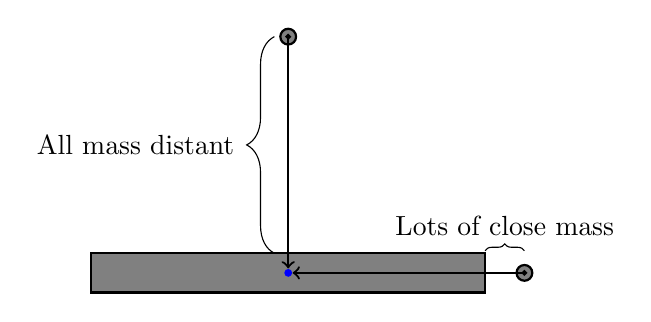
\begin{tikzpicture}
      \tikzmath{
        \h = 0.5;
        \w = 5;
        \rDot = 0.02;
        \rSat = 0.1;
        \r = 3;
      }

      \coordinate (P) at (\w / 2, \h /2 + \r);
      \coordinate (E) at (\w / 2 + \r, \h / 2);

      
      \draw[black, thick, fill=gray] rectangle (\w,\h);

      \filldraw[black, thick, fill=gray] (E) circle [x radius = \rSat, y radius = \rSat];
      \filldraw[black, thick, fill=gray] (P) circle [x radius = \rSat, y radius = \rSat];
      \filldraw[black, thick] (E) circle [x radius = \rDot, y radius = \rDot]; 
      \filldraw[black, thick] (P) circle [x radius = \rDot, y radius = \rDot]; 

      \node[circle,fill=blue,inner sep=1pt,minimum size=\rDot] (C) at (\w / 2, \h / 2) {};
      
      \draw[black,thick,->] (E) -- (C);
      \draw [decorate,decoration={brace,mirror,raise=8pt}]
      (E) -- (\w, \h / 2) node[midway,yshift=10pt,above]{Lots of close mass};
      
      \draw[black,thick,->] (P) -- (C);
      \draw [decorate,decoration={brace,amplitude=10pt,mirror,raise=5pt}]
      (P) -- (\w / 2, \h) node[midway,xshift=-16pt,left]{All mass distant};
    \end{tikzpicture}
  \end{center}

  Equatorial gravity increases. Polar gravity decreases.
\end{frame}


\begin{frame}{Perturbation: Indirect Oblation}
  \[ \ddot{R} = \ddot{R}_\text{2B} + \ddot{R}_\text{PM} + \ddot{R}_\text{NS}  + \ddot{R}_\text{IO}\]
  \begin{itemize}
  \item Earth is not an inertial reference frame
    \begin{itemize}
    \item Has its own orbit around Sol
    \item Yanked around by Luna inside that orbit
    \end{itemize}
  \item ``Shaky Camera'' effect
  \end{itemize}
\end{frame}

\begin{frame}{Perturbation: Drag}
  \[ \ddot{R} = \ddot{R}_\text{2B} + \ddot{R}_\text{PM} + \ddot{R}_\text{NS}  + \ddot{R}_\text{IO} + \ddot{R}_\text{D} \]

  \begin{itemize}
  \item Drag equation: $F_\text{D} = \frac{1}{2}\rho v^2 C_\text{D} A$
  \item Scales by
    \begin{itemize}
    \item Object shape and orientation ($C_\text{D}, A$).
    \item Square of object velocity $v^2$.
    \item Atmospheric density $rho$, drops ~exponentially with altitude.
    \end{itemize}
  \item LEO objects (altitude < 2000 km) are low and fast
    \begin{itemize}
    \item experience non-negligible drag
    \end{itemize}
  \item Bonus: non-periodic and non-conservative.
  \end{itemize}
\end{frame}

\begin{frame}{Perturbation: Solar Radiation Pressure}
  \[ \ddot{R} = \ddot{R}_\text{2B} + \ddot{R}_\text{PM} + \ddot{R}_\text{NS}  + \ddot{R}_\text{IO} + \ddot{R}_\text{D} + \ddot{R}_\text{SRP}\]

  \begin{itemize}
  \item $\gamma := \sqrt{\frac{c^2}{c^2 - v^2}}$
  \item $ p = \gamma m v$
  \item photons: $m\rightarrow0, \gamma \rightarrow \infty $
    \begin{itemize}
    \item $p \rightarrow ?$
    \item God's math: $ p = \frac{h}{\lambda} $
    \end{itemize}
  \item Absorbing and emitting light imparts momentum
    \begin{itemize}
    \item Sunlight never stops: SRP
    \item Most impactful on higher altitude orbits
    \item Non-periodic and non-conservative
    \end{itemize}
  \end{itemize}
\end{frame}

\begin{frame}{Perturbation: Thrust}
  \[ \ddot{R} = \ddot{R}_\text{2B} + \ddot{R}_\text{PM} + \ddot{R}_\text{NS}  + \ddot{R}_\text{IO} + \ddot{R}_\text{D} + \ddot{R}_\text{SRP} + \ddot{R}_\text{T} \]

  \begin{itemize}
  \item Orbital payloads commonly come equipped with maneuvering thrusters
    \begin{itemize}
    \item Chemical burns (fast, short)
    \item Electric propulsion (slow, long)
    \end{itemize}
  \item Good news: allows for doing something about predicted collisions
  \item Bad news: Non-periodic, non-conservative, AND non-physical(-ish)
  \end{itemize}
\end{frame}

\begin{frame}{Perturbation Impacts}
  \begin{itemize}
  \item Low-to-medium fidelity diff-eqs can be solved analytically
    \begin{itemize}
      \item E.g. Brouwer models, SGP4/SDP4
    \end{itemize}
  \item High-fidelity generally resort to numerical integration
    \begin{itemize}
      \item E.g. NORAD Special Perturbations (SP)
    \end{itemize}
  \item Low- and high-fidelity models can diverge significantly, rapidly
    \begin{itemize}
    \item By kilometers
    \item Within a few orbital periods (i.e. hours)
    \end{itemize}
  \end{itemize}
\end{frame}

\subsection{Consequence}

\begin{frame}{Mission Safety}
  \[ E(\text{Cost}(X)) = P(X) \cdot \text{Cost}(X) \]
  
  \begin{itemize}
  \item Plausible $\text{Cost}(X)$: 100 million USD
  \item Plausible $P(X)$: 2e-4
  \item $E(\text{Cost}(X)) = 2 \cdot 10^{-4} \cdot 10^8 = 20000$ USD
    \begin{itemize}
    \item Might be worth mitigating
    \item Although, $\sim 85\%$ of likely-lethal conjunctors aren't even
      tracked \ldots
    \end{itemize}
  \end{itemize}
\end{frame}

\begin{frame}{Domain Safety I}

  \begin{itemize}
  \item Orbit contention is self-reinforcing
    \begin{itemize}
    \item More objects means more conjunctions
    \item More conjunctions means more collisions
    \item More collisions means more objects
    \end{itemize}
  \item Critical density $\rightarrow$ runaway, sustained fragmentation
    \begin{itemize}
    \item Kessler syndrome
    \end{itemize}
  \item Sub-critical density increases still increase hazard to ecosystem
  \end{itemize}
\end{frame}

\begin{frame}{Domain Safety II}
  \begin{itemize}
  \item Vested public interest in controlling flux
  \item Must avoid collisions, especially between large objects
    \begin{itemize}
    \item Debris potential strongly linked to object size
    \item Largest objects are best tracked
    \item Objects follow a power-law distribution: many, many small pieces,
      comparatively few large
    \end{itemize}
  \end{itemize}
\end{frame}

\section{Conjunction Identification}
\subsection{Volumetric Screening}

\begin{frame}{Conjunction Screening}
  \begin{itemize}
  \item Before a conjunction can be analyzed it must be identified
    \begin{itemize}
    \item Want to know the time of closest approach (TCA)
    \item and of course the conjunctors' states at TCA
    \end{itemize}
  \item Technically not a CARA responsibility
    \begin{itemize}
    \item Screening computed for CARA by CSpOC using COMBO (Computation of Miss
      Between Orbits).
    \item Operates on a ``flying-ellipsoid'' volumetric screening paradigm.
    \end{itemize}
  \end{itemize}
\end{frame}

\begin{frame}[fragile]{Volumetric Screening}
  \begin{center}
    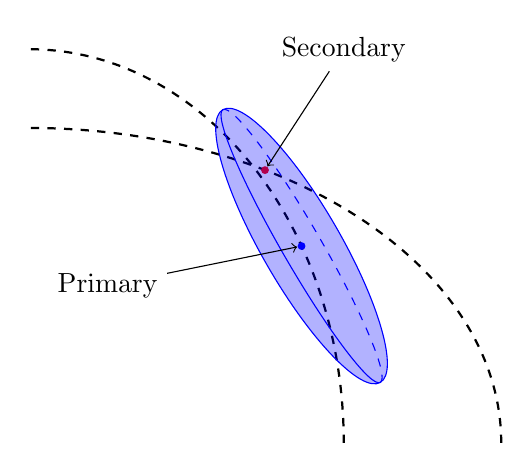
\begin{tikzpicture}
      \tikzmath{
        \rDot = 0.04;
      }

      
      \coordinate (P) at (30:4 and 5);
      \draw[black, thick, dashed] (0:4 and 5) arc (0:90:4 and 5);
      \node[circle,fill=blue,inner sep=1pt,minimum size=\rDot] (PN) at (P) {};
      
      \coordinate (S) at (60:6 and 4);
      \draw[black, thick, dashed] (0:6 and 4) arc (0:90:6 and 4);
      \node[circle,fill=red,inner sep=1pt,minimum size=\rDot] (SN) at (S) {};

      \draw[blue, rotate=30, fill=blue, fill opacity=.30] (P) circle (0.5 and 2);
      \draw[blue, rotate=30, shift=(P)] (0, 2) arc (90:270:0.25 and 2);
      \draw[blue, dashed, rotate=30, shift=(P)] (0, -2) arc (-90:90:0.25 and 2);

      \node (PLabel) at (1,2) {Primary};
      \node (SLabel) at (4,5) {Secondary};

      \draw[black, ->] (PLabel) -- (PN);
      \draw[black, ->] (SLabel) -- (SN);
    \end{tikzpicture}
  \end{center}
\end{frame}

\begin{frame}{Volumetric Screening}
  \begin{algorithmic}
    \Procedure{ScreenConjunctions}{}
    \For{$p, s, t \in \textit{Primaries} \times \textit{Secondaries} \times \textit{Time Slices}$}
      \State $V \gets \text{ellipse around }p(t)$
      \If{$s(t).\text{pos} \notin V$}
        \State \textbf{continue}
      \EndIf
      \State $d(\tau) := || p(\tau).\text{pos}  - s(\tau).\text{pos} ||$
      \If{$\text{sign}(d'(t)) = \text{sign}(d'(t+\Delta t))$}
        \State \textbf{continue}
      \EndIf
      \State $t^* \gets \operatorname*{argmin}_{[t, t + \Delta t]} d$
      \State $\text{Emit } (p, s, t^*)$
    \EndFor
    \EndProcedure  
  \end{algorithmic}
\end{frame}

\section{Conjunction Analysis}
\subsection{Risk Measures}

\begin{frame}{Standoff Distance}
  \begin{itemize}
  \item Most intuitive measure of safety
    \begin{itemize}
    \item If we are far apart, of course we aren't touching.
    \item Implicitly part of volumetric screening regimes.
    \end{itemize}

  \item Difficult to map distance onto risk.
    \begin{itemize}
    \item How far apart is far? Meters? Kilometers?
    \end{itemize}
    
  \item Cannot capture uncertainty
    \begin{itemize}
    \item What if our measurements of a satellite's state are known to be imprecise?
    \end{itemize}
    
  \item Tendency toward conservatism
    \begin{itemize}
      \item sometimes desirable, e.g. around human space flight assets
    \end{itemize}
  \end{itemize}
\end{frame}

\begin{frame}{Probability of Collision}
  \begin{itemize}
  \item Most commonly used measure of safety.

  \item Answers the challenges with standoff distance
    \begin{itemize}
    \item Maps naturally to risk.
    \item Captures and describes uncertainty and imprecision.
    \item Allows for mindfully tuned risk postures.
    \end{itemize}

  \item But! Can suffer from probability dilution.
    \begin{itemize}
    \item Space is big. Really big. Really, really big.
    \item Rubbish measurements $\Rightarrow P_C \approx 0$.
    \item Probability is ``diluted'' across space.
    \end{itemize}
  \end{itemize}
\end{frame}

% TODO: roll this into motivation section
% TODO: Add a slide+subsection for MTS
\begin{frame}{Severity Estimation}
  \begin{itemize}
  \item For the domain:
    \begin{itemize}
    \item Different collisions create different amounts of debris.
    \item EVOLVE: empirically determined model mapping relative masses and
      velocities to expected fragmentation count.
    \item Basic rules: fast is bad, heavy is bad.
    \item Of course, ultimately dependent on O/Os to maneuver/mitigate.
    \end{itemize}

  \item For O/Os:
    \begin{itemize}
    \item Everything is moving too damned fast
    \item Everything is too damned expensive
    \item A hit is a hit is a hit is a bad time
    \end{itemize}
  \end{itemize}
\end{frame}

\subsection{2D $P_C$}
\begin{frame}{Naive $P_C$}

  \[ \int\int f(S_1,S_2) \mathbb{I}(\text{collision} | S_1,S_2) dS_1 dS_2 \]

  \begin{itemize}
  \item That's a 12-dimensional integral.
  \item $\mathbb{I}(\text{collision} | S_1,S_2)$ is a nightmare function.
  \item Let's make some simplifying assumptions
  \end{itemize}
\end{frame}

\begin{frame}{2D $P_C$: Assumptions}
  \begin{enumerate}
  \item State position vectors $R_1 \sim \mathcal{N}(\bar{R_1}, C_1), R_2 \sim \mathcal{N}(\bar{R_2}, C_2)$
  \item $R_1 \perp R_2$
  \item Velocity uncertainty is negligible
  \item Position uncertainty is stable throughout the encounter
  \item Relative motion is linear throughout the encounter
  \item Both objects are spheres
  \end{enumerate}
\end{frame}

\begin{frame}{2D $P_C$}
  Core idea: Don't think about two objects, think about
  the distance separating them. More precisely, let
  
  \[ R_\text{miss} := R_2 - R_1 \]

  We wish to integrate

  \[ \int f_\text{miss}(R) \mathbb{I}(\text{collision} | R) dR \]
\end{frame}

\begin{frame}{2D $P_C$}

  \[ \int \alert{f_\text{miss}(R)} \mathbb{I}(\text{collision} | R) dR \]

  Recall: $R_1 \perp R_2$, both Gaussian. So

  \[ R_\text{miss} \sim \mathcal{N}(\bar{R_2} - \bar{R_1}, C_2 - C_1) \]

  $f_\text{miss}$ is just $\phi$!
\end{frame}


\begin{frame}{2D $P_C$}

  \[ \int f_\text{miss}(R) \alert{\mathbb{I}(\text{collision} | R)} dR \]

  Linear motion, spherical objects. Collision iff $\exists t \in \mathbb{R}$ s.t.

  \[ ||R_\text{miss} + v_\text{miss} \cdot t|| < r \]

  That's a cylinder!

  % TODO: insert image here
\end{frame}


\begin{frame}{2D $P_C$}
  Observe: cylinder is infinite. Rotate our $z$-axis to align with it, and it
  will marginalize to 1.

  % TODO: insert image here

  A little final massaging and we arrive at a numerical-quadrature-friendly
  integral.
  
  \[ P_C = \frac{1}{\sqrt{\det(2\pi C)}} \int\int_A \exp \left( -\frac{r^TC^{-1}r}{2}\right)dxdy \]
\end{frame}

\subsection{3D $P_C$}

\begin{frame}{Hyperkinetic Assumptions}
  \begin{itemize}
  \item 2D $P_C$ treated conjunctors like a pair of bullets
  \item Pretty good model when relative velocity is high, encounter is short
  \item Not all close approaches occur at high (relative) velocity, though
  \item Can we do better?
  \end{itemize}
\end{frame}

\begin{frame}{3D $P_C$}
  What happens if we trace our miss vector through the encounter?

  \[ \int P(\text{conjunctors touching at }t) dt\]

  That's actually $N_C$, the expected number of collisions, but close enough.
\end{frame}


\begin{frame}{3D $P_C$}
  \[ P(\text{conjunctors touching at }t) = P(||R_\text{miss}(t)|| = r) \]

  \begin{itemize}
  \item The integrand is a surface integral over a sphere!
    \begin{itemize}
    \item Total integration dimension: 3
    \item Curse of dimensionality remains weak
    \end{itemize}
  \item Can we compute and integrate $R_\text{miss}(t)$?
    \begin{itemize}
    \item Yes, with two-body equations of motion\ldots but the math is kind of
      involved.
    \item Please read the full pub if interested.
    \end{itemize}
  \end{itemize}
\end{frame}


\subsection{Monte Carlo}

\begin{frame}{Motivation}
  \begin{itemize}
  \item All this integration, it's making my head hurt.
  \item Even the fancy 3D $P_C$ variant had to make simplifying assumptions.
  \item This is a stochastic process, let's try modeling it stochastically.
  \end{itemize}
\end{frame}

\begin{frame}{From-Epoch MC}
  \begin{algorithmic}
    \Procedure{FromEpochMC}{\textit{primOD}, \textit{secOD}, \textit{trials}}
    \State $\textit{hits} \gets 0$
    \For{$i \in [0,\ldots,\textit{trials})$}
      \State $p \gets \text{draw from } \textit{primOD}$ 
      \State $s \gets \text{draw from } \textit{secOD}$
      \If{$p.\text{propagate()} \text{ collides with } s.\text{propagate()}$}
        \State $\textit{hits} \gets \textit{hits} + 1$
      \EndIf
      \EndFor
    \State \Return $\frac{\textit{hits}}{\textit{trials}}$
    \EndProcedure  
  \end{algorithmic}
\end{frame}

\begin{frame}{From-Epoch MC}
  \begin{itemize}
  \item No simplifying assumptions! Estimate is as good as
    \begin{itemize}
    \item Our orbit propagation algorithm
    \item The number of trials we run
    \end{itemize}
  \item Heinously expensive, though
    \begin{itemize}
    \item Millions and millions of trials
    \item Each trial doing high-fidelity numerical ODE solving from epoch up
      through TCA
    \end{itemize}
  \item Most useful to prove out the accuracy of other algorithms.
  \end{itemize}
\end{frame}

\begin{frame}{From-TCA MC}
  \begin{algorithmic}
    \Procedure{FromTCAMC}{\textit{primTCA}, \textit{secTCA}, \textit{trials}}
    \State $\textit{hits} \gets 0$
    \For{$i \in [0,\ldots,\textit{trials})$}
      \State $p \gets \text{draw from } \textit{primTCA}$ 
      \State $s \gets \text{draw from } \textit{secTCA}$
      \If{$p.\text{propForward()} \text{ collides with } s.\text{propForward()}$}
        \State $\textit{hits} \gets \textit{hits} + 1$
      \ElsIf{$p.\text{propBack()} \text{ collides with } s.\text{propBack()}$}
        \State $\textit{hits} \gets \textit{hits} + 1$
      \EndIf
      \EndFor
    \State \Return $\frac{\textit{hits}}{\textit{trials}}$
    \EndProcedure  
  \end{algorithmic}
\end{frame}

\begin{frame}{From-TCA MC}
  \begin{itemize}
  \item Faster than From-Epoch
    \begin{itemize}
    \item Only need to propagate motion around the encounter
    \item Shorter motion-prop window means lower fidelity propagation schemes
      can be used.
    \end{itemize}
  \item Depends on assumptions about the shape of propagated uncertainty
    \begin{itemize}
    \item Not really a practical issue if we're careful to sample in curvilinear
      coordinates.
    \end{itemize}
  \item Still much slower than analytic methods.
    \begin{itemize}
    \item Empirically not much better results
    \item Not frequently used in CARA in practice
    \end{itemize}
  \end{itemize}
\end{frame}


%% Q&A and Further reading.
\miniframesoff
\section*{}
\begin{frame}{References}[allowframebreaks]
  \tiny
% TODO
%    \printbibliography
\end{frame}

\begin{frame}{Self Link}
  The source for this presentation is hosted at
\url{https://github.com/alan-christopher/cara-edu}.

\end{frame}
\end{document}
